% !TeX spellcheck = nl_NL
\documentclass[a4paper,kul]{kulakarticle} %options: kul or kulak (default)

\usepackage[utf8]{inputenc}
\usepackage[dutch]{babel}

\date{Academiejaar 2021 -- 2022}
\address{
	Industriële Ingenieurswetenschappen \\
	Trillingen \& Golven \\
	Maarten Vanierschot}
\title{Afleidingen}
\author{Robbe Decapmaker}
\usepackage{hyperref}
\usepackage{graphicx}
\usepackage{amsmath, amssymb, amsthm}
\usepackage{siunitx}
\usepackage{flafter} 
\usepackage{pdfpages}
\usepackage{pgfplots}


\begin{document}

\maketitle

\section*{Inleiding}

De afleidingen voor trillingen en golven. \href{https://github.com/debber1/Afleidingen_TG}{De source code is te vinden op github.}\\
%DEZE ZIN IS ENKEL RELEVANT TIJDENS DE ONTWIKKELING VAN DIT DOCUMENT
\textbf{Dit document is een `work in progress', dit wil zeggen dat er (ongeveer) een wekelijkse update zal zijn. De meest recente versie zal altijd op Github staan!}

\section{Afleiding 1}

\textbf{Afleiding van de uitdrukking voor de verplaatsing van een ongedempte trilling aan de hand van de bewegings-vergelijking}\\
\begin{figure}[htbp]
	\centering
	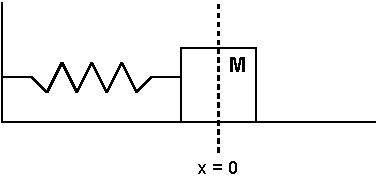
\includegraphics[width=0.4\linewidth]{MassaVeer}
	\caption[Massa veer systeem]{Massa veer systeem}
	\label{fig:massaveer}
\end{figure}
\begin{figure}[htbp]
	\centering
	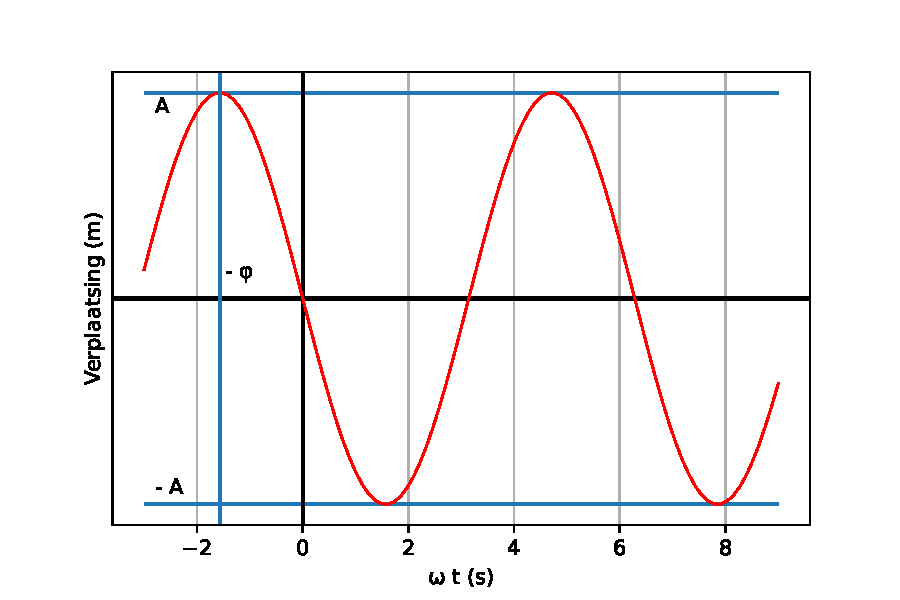
\includegraphics[width=0.7\linewidth]{Harmonische_Oscillator}
	\caption[Harmonische Oscillator]{Harmonische Oscillator}
	\label{fig:harmonischeoscilator}
\end{figure}

We stellen eerst de tweede wet van Newton op voor het blokje M uit figuur \ref{fig:massaveer}.
\begin{equation*}
	\sum \vec{F} = m\vec{a}
\end{equation*}
We kijken nu enkel naar de x-component, en brengen we de kracht van de veer in rekening:
\begin{equation*}
	-kx = m\frac{d^2x}{dt^2}
\end{equation*}
We hebben ook de versnelling geschreven als de tweede afgeleide van de verplaatsing. Door alle termen naar het linker lid te verplaatsen krijgen we volgende differentiaal vergelijking: 
\begin{equation}
	m\frac{d^2x}{dt^2} + kx = 0
	\label{eq:DVGLTrilling}
\end{equation}
Deze differentiaal vergelijking moeten we oplossen aan de hand van beginvoorwaarden. Deze voorwaarden verkrijgen we experimenteel. Bij het experiment noteren we de uitwijking tegenover de tijd. Hierdoor verkrijgen we figuur \ref{fig:harmonischeoscilator}.
Wiskundig vertaalt dit zich tot: 
\begin{equation}
	x(t) = A cos(\omega t + \varphi)
	\label{eq:trilling}
\end{equation}
we kunnen vergelijking \ref{eq:trilling} afleiden om de snelheid van het blokje te verkrijgen: 
\begin{equation}
	v(t) = \frac{dx(t)}{dt} = -\omega Asin(\omega t + \varphi)
	\label{eq:trillingsnelheid}
\end{equation}
Door nogmaals vergelijking \ref{eq:trillingsnelheid} nogmaals af te leiden kunnen we ook de versnelling van het blokje verkrijgen:
\begin{equation}
	a(t) = \frac{d^2x(t)}{dt^2} = -\omega^2 Acos(\omega t + \varphi)
	\label{eq:trillingversnelling}
\end{equation}
Nu kunnen we vergelijkingen \ref{eq:trillingversnelling} en \ref{eq:trilling} invullen in vergelijking \ref{eq:DVGLTrilling}:
\begin{equation}
	-\omega^2 mAcos(\omega t + \varphi) + k A cos(\omega t + \varphi) = 0
	\label{eq:Bewegingsvergelijking}
\end{equation}
Vergelijking \ref{eq:Bewegingsvergelijking} is nu een oplossing voor differentiaal vergelijking \ref{eq:DVGLTrilling} als aan volgende voorwaarde voldaan is:
\begin{align*}
	-\omega^2 mAcos(\omega t + \varphi) + k A cos(\omega t + \varphi) & = 0\\
	(\frac{k}{m}-\omega^2)A cos(\omega t + \varphi) & = 0\\
	\frac{k}{m}-\omega^2 & = 0\\
	\frac{k}{m} & = \omega^2
\end{align*}


\newpage
\section{Afleiding 2}
\textbf{Afleiding van de potentiële en kinetische energie van een ongedempte trilling in functie van de plaats}
\\

Er zijn 2 vormen van energie aanwezig in een massa-veer-systeem. We hebben de potentiële energie in de veer en de kinetische energie van het blokje.
\begin{align*}
	E = & \frac{1}{2}kx^2 + \frac{1}{2}mv^2\\
	E(x) = & \frac{1}{2}k A^2cos^2(\omega t +\varphi) + \frac{1}{2}m \omega^2 A^2 sin^2(\omega t + \varphi)\\
	E(x) = & \frac{1}{2}k A^2cos^2(\omega t +\varphi) + \frac{1}{2}m \frac{k}{m} A^2 sin^2(\omega t + \varphi)\\
	E(x) = & \frac{1}{2} k A^2 (cos^2(\omega t +\varphi) + sin^2(\omega t + \varphi))\\
	E(x) = & \frac{1}{2} k A^2
\end{align*} 
We zien nu duidelijk dat de hoeveelheid energie niet afhankelijk is van de uitwijking van de massa. Met andere woorden, de energie blijft constant in het systeem (Figuur \ref{fig:energiebalans}).
\begin{figure}[htbp]
	\centering
	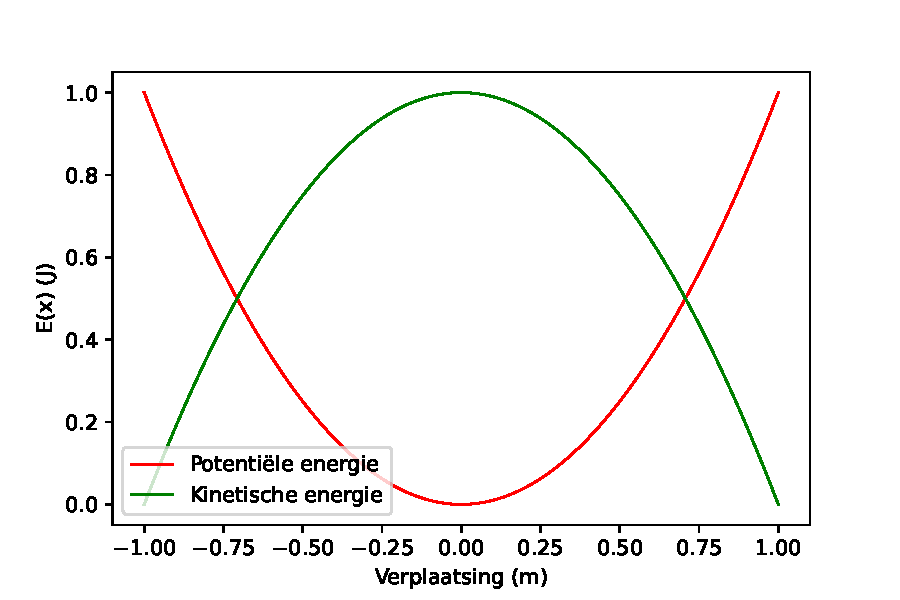
\includegraphics[width=0.7\linewidth]{Energie_Balans}
	\caption[Energie balans]{Energie balans}
	\label{fig:energiebalans}
\end{figure}

\newpage

\section{Afleiding 3}
\textbf{Snelheid in functie van de afstand}
\begin{equation*}
	\frac{dv}{dt} = \frac{dv}{dx}\cdot\frac{dx}{dt}
\end{equation*}
We kunnen vergelijkingen \ref{eq:trilling} en \ref{eq:trillingsnelheid} invullen:
\begin{equation*}
	-A\omega^2cos(\omega t + \varphi) = \frac{dv}{dx}\cdot A\omega sin(\omega t +\varphi)
\end{equation*}
Na schrappen en herschikken:
\begin{equation*}
	\frac{dv}{dx} = \frac{\omega cos(\omega t + \varphi)}{sin(\omega t + \varphi)}
\end{equation*}
Sinus substitutie:
\begin{align*}
	\frac{dv}{dx} =& \frac{\omega cos(\omega t + \varphi)}{\sqrt{1-cos^2(\omega t + \varphi)}}\\
	\frac{dv}{dx} =& \frac{\pm \omega \frac{x}{A}}{\sqrt{1-\frac{x^2}{A^2}}}
\end{align*}
Nu integratie van beide leden:
\begin{equation*}
	\int dv = \int \frac{\pm \omega \frac{x}{A}}{\sqrt{1-\frac{x^2}{A^2}}} dx
\end{equation*}
De snelheid in functie van de afstand is dus:
\begin{equation}
	\label{eq:snelheid_positie}
	v(x) = \omega A\sqrt{1-\frac{x^2}{A^2}}
\end{equation}
Uit vergelijking \ref{eq:snelheid_positie} kunnen we nu ook afleiden wat de uitdrukking is voor $v_{\text{max}}$. We weten dat $v_{\text{max}}$ zich zal voordoen bij het evenwichtspunt oftewel als x = 0.
\begin{align*}
	v(x) =& \omega A\sqrt{1-\frac{x^2}{A^2}}\\
	v_{\text{max}} =& \omega A\sqrt{1-\frac{0^2}{A^2}}\\
	v_{\text{max}} =& \omega A\sqrt{1}\\
	v_{\text{max}} =& \omega A
\end{align*}
\newpage
\section{Afleiding 4}
\textbf{Afleiding van de beweging van een pendulum aan de hand van de bewegingsvergelijking}
\begin{figure}[htbp]
	\centering
	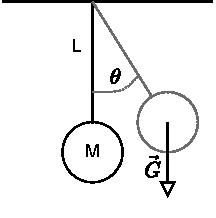
\includegraphics[width=0.5\linewidth]{Pendulum}
	\caption[Pendulum]{Pendulum}
	\label{fig:pendulum}
\end{figure}
De drijvende kracht van de pendulum is gelijk aan:
\begin{equation*}
	F = -mg sin(\theta)
\end{equation*}
Hiermee kunnen we de bewegingsvergelijking opstellen:
\begin{equation*}
	m\frac{d^2x}{dt^2} = -mgsin(\theta)
\end{equation*}
We kunnen stellen dat $sin(\theta) \approx \theta$ voor een kleine $\theta$:
\begin{equation*}
	m\frac{d^2x}{dt^2} = -mg\theta
\end{equation*}
We kunnen ook stellen dat $x = l\theta$:
\begin{equation*}
	ml\frac{d^2\theta}{dt^2} = -mg\theta
\end{equation*}
We kunnen dit nu herschrijven naar:
\begin{equation*}
	\frac{d^2\theta}{dt^2} +\frac{g}{l}\theta = 0
\end{equation*}
Dit geeft ons een differentiaalvergelijking. Een oplossing ziet er als volgt uit:
\begin{equation*}
	\theta (t) = \theta_0 cos(\omega t +\varphi)
\end{equation*}
Hierbij zien we dat $\omega = \sqrt{\frac{g}{l}}$.
\newpage
\section{Afleiding 5}
\textbf{Gedempte harmonische trilling}\\
\begin{figure}[htbp]
	\centering
	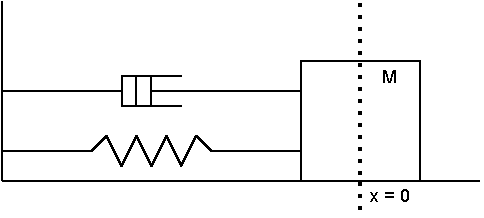
\includegraphics[width=0.7\linewidth]{DempingVeer}
	\caption[Gedempt massa veer systeem]{Gedempt massa veer systeem}
	\label{fig:dempingveer}
\end{figure}
We beginnen met de bewegingsvergelijking op te stellen:
\begin{align*}
	m \vec{a} =& \vec{F}_{veer} + \vec{F}_{demper}\\
	m \frac{d^2x}{dt^2} = & -kx - bv\\
	m \frac{d^2x}{dt^2} = & -kx - b\frac{dx}{dt}\\
	0 = & m \frac{d^2x}{dt^2} + b\frac{dx}{dt} + kx
\end{align*}
We maken gebruik van de formule van Euler $e^{i\varphi}=cos(\varphi) +isin(\varphi)$ om tot een oplossing van de differentiaalvergelijking te komen:
\begin{equation*}
	\widetilde{x}(t) = Ae^{(\gamma +i\omega)t+i\varphi}
\end{equation*}
Het reëel deel is dus:
\begin{equation*}
	x(t) = Re(\widetilde{x}(t)) = Ae^{\gamma t}cos(\omega t + \varphi)
\end{equation*}
We kunnen deze nu invullen in de bewegingsvergelijking:
\begin{equation}
	\label{eq:complexbeweging}
	m(\gamma +i\omega)^2\widetilde{x}(t) + b(\gamma +i\omega)e^{(\gamma +i\omega)t+i\varphi}+ke^{(\gamma +i\omega)t+i\varphi} = 0
\end{equation}
Na herordenen en het delen door m, krijgen we:
\begin{equation*}
	\gamma^2+2i\gamma\omega-\omega^2+\frac{b}{m}\gamma+i\frac{\omega b}{m}+\frac{k}{m}=0
\end{equation*}
We kijken nu naar het imaginair deel:
\begin{align*}
	2i\gamma \omega +i\frac{\omega b}{m}&=0\\
	2\gamma + \frac{b}{m} = 0\\
	-\frac{b}{2m} = \gamma
\end{align*}
We vullen nu deze waarde van $\gamma$ in in het reëel deel van vergelijking \ref{eq:complexbeweging}:
\begin{align*}
	\gamma^2-\omega^2+\frac{b}{m}\gamma+\frac{k}{m} &=0\\
	(-\frac{b}{2m})^2-\omega^2+\frac{b}{m}(-\frac{b}{2m})+\frac{k}{m} &=0\\ 
	\frac{k}{m}-\frac{b^2}{4m^2}&=\omega^2\\
	\sqrt{\frac{k}{m}-\frac{b^2}{4m^2}}&=\omega
\end{align*}
Hiermee hebben we nu de natuurlijke frequentie van het systeem gevonden. We kunnen tot slot ook nog stellen dat:
\begin{equation*}
	x(t) = Re(\widetilde{x}(t)) = Ae^{-\frac{b}{2m} t}cos(\omega t + \varphi)
\end{equation*}
We kunnen nu drie gevallen onderscheiden: 
\begin{figure}[htbp]
	\centering
	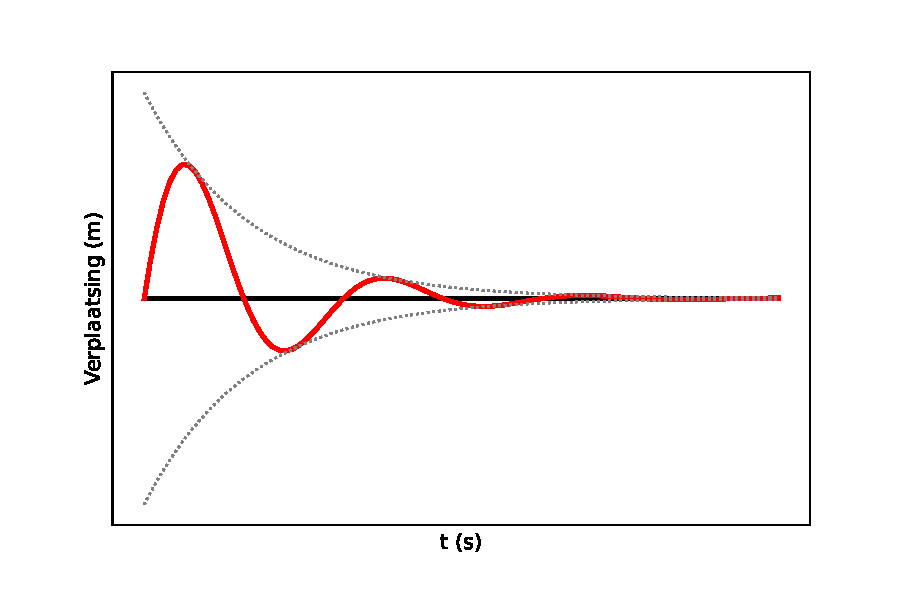
\includegraphics[width=0.6\linewidth]{Ondergedempt}
	\caption[Ondergedempte trilling]{Ondergedempte trilling ($b^2 << 4mk$)}
	\label{fig:ondergedempt}
\end{figure}
\begin{figure}[htbp]
	\centering
	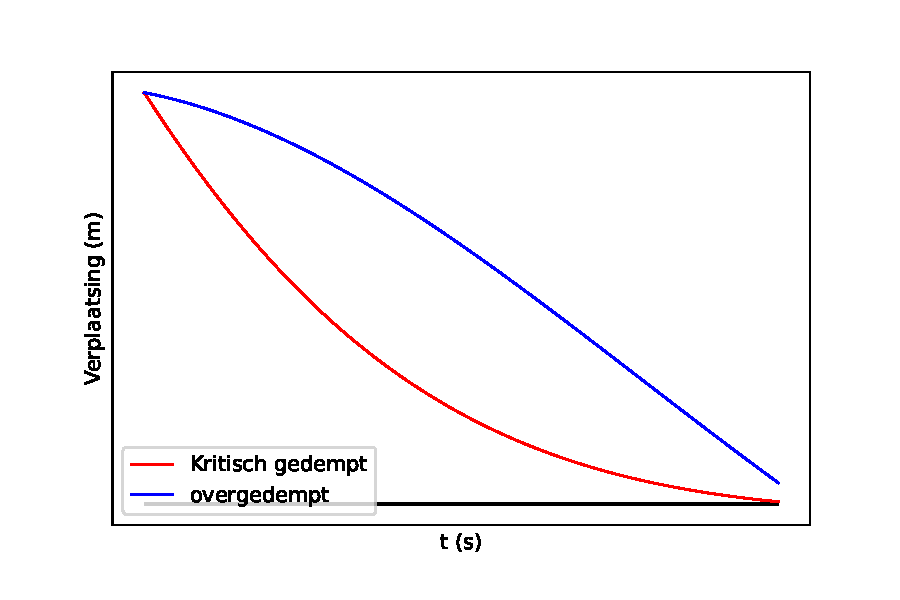
\includegraphics[width=0.6\linewidth]{Over_Kritisch_gedempt}
	\caption[Kritisch en over gedempte trilling]{Kritisch ($b^2 = 4mk$) en over gedempte ($b^2 >> 4mk$) trilling}
	\label{fig:overkritischgedempt}
\end{figure}


\newpage
\section{Afleiding 6}
\textbf{Gedwongen trillingen}\\
We stellen eerst de bewegingsvergelijking op:
\begin{equation}
	m\frac{d^2\widetilde{x}(t)}{dt^2}+b\frac{d\widetilde{x}(t)}{dt}+k\widetilde{x}(t) = F_0cos(\omega t)
	\label{eq:gedwongenbewegings}
\end{equation}
Een voorstel voor de algemene oplossing van differentiaalvergelijking \ref{eq:gedwongenbewegings} ziet er als volgt uit:
\begin{equation*}
	\widetilde{x}(t) = Ae^{i(\omega t +\varphi)}
\end{equation*}
waarbij $\widetilde{F} = F_0e^{i\omega t}e^{-i\varphi}$.
Dit kunnen we nu invullen in vergelijking \ref{eq:gedwongenbewegings}:
\begin{align*}
	m\omega^2\widetilde{x}(t)+i\omega b\widetilde{x}(t)+k\widetilde{x}(t) & =F_0e^{i\omega t}e^{-i\varphi}\\
	m\omega^2A^{i\omega t}e^{i\varphi}+i\omega bA^{i\omega t}e^{i\varphi}+kA^{i\omega t}e^{i\varphi} & =F_0e^{i\omega t}e^{-i\varphi}\\
	m\omega^2A+i\omega b+k & =F_0e^{-i\varphi} 
\end{align*}
We kunnen dit opsplitsen in een imaginair en reëel deel:
\begin{description}
	\item[Imaginair:]$\omega bA = -F_0sin(\varphi)$
	\item[Reëel:] $-m\omega A +kA = F_0cos(\varphi)$
\end{description}
Als we nu het imaginair deel delen door het reëel deel verkrijgen we voor $\varphi$:
\begin{align*}
	-\frac{\omega b}{k-m\omega^2} &= tan(\varphi)\\
	bgtan(\frac{-\omega b}{k-m\omega^2}) & =\varphi
\end{align*}
Om de amplitude te bepalen kijken we opnieuw naar het imaginair deel:
\begin{align*}
	\omega bA &= -F_0sin(\varphi)\\
	\omega bA &= -F_0\frac{tan(\varphi)}{\sqrt{1+tan^2(\varphi)}}\\
	\omega bA &= -F_0\frac{tan(bgtan(\frac{-\omega b}{k-m\omega^2}))}{\sqrt{1+tan^2(bgtan(\frac{-\omega b}{k-m\omega^2}))}}\\
	\omega bA &= -F_0\frac{\frac{-\omega b}{k-m\omega^2}}{\sqrt{1+\frac{\omega^2 b^2}{(k-m\omega^2)^2}}}\\
	\omega bA &= -F_0\frac{\frac{-\omega b}{k-m\omega^2}}{\sqrt{\frac{(k-m\omega^2)^2+\omega^2 b^2}{(k-m\omega^2)^2}}}\\
	A &= \frac{\frac{F_0}{k-m\omega^2}}{\sqrt{\frac{(k-m\omega^2)^2+\omega^2 b^2}{(k-m\omega^2)^2}}}\\
	A &= \frac{\frac{F_0}{m}}{\sqrt{(\frac{k}{m}-\omega^2)^2+\frac{\omega^2b^2}{m^2}}}\\
	A &= \frac{\frac{F_0}{m}}{\sqrt{(\omega_0^2-\omega^2)^2+\frac{\omega^2b^2}{m^2}}}	
\end{align*}
met $\omega_0$ de natuurlijke frequentie van het systeem en $\omega$ de gedwongen frequentie.
\newpage
\section{Afleiding 7}
\textbf{Golf vergelijking}\\
We nemen aan da $F_r$ en $F_l$ uit figuur \ref{fig:touwgolf} gelijk zijn aan elkaar en aan de spanning in het touw $\sigma A$. we stellen ook dat de massa voldoet aan $dm=\rho dsA$.\\
\begin{figure}[htbp]
	\centering
	\includegraphics[width=0.7\linewidth]{"touw_golf"}
	\caption[Touw]{Touw}
	\label{fig:touwgolf}
\end{figure}\\
We starten met het opstellen van de wet van Newton:
\begin{align*}
	\sum\vec{F}&=m\vec{a}\\
	F_rsin(\alpha_r) & = F_lsin(\alpha_l) = dma_y\\
	\sigma A(sin(\alpha_r)-sin(\alpha_l)) & = dm\frac{\partial^2y}{\partial t^2}\\
	\sigma(\frac{dy}{dx}|_r-\frac{dy}{dx}|_l) & = \rho ds \frac{\partial^2y}{\partial t^2}
\end{align*}
We stellen dat $\alpha$ klein is, en dus kunnen we zeggen dat $sin(\alpha)\approx tan(\alpha) = \frac{dx}{dy}$. We nemen ook aan dat $ds \approx dx$.
\begin{align*}
	\sigma\frac{\frac{dy}{dx}|_r-\frac{dy}{dx}|_l}{dx} & = \rho \frac{\partial^2y}{\partial t^2}\\
	\sigma\frac{\partial^2y}{\partial x^2} & = \rho \frac{\partial^2y}{\partial t^2}\\
	\frac{\partial^2y}{\partial t^2} & = \frac{\sigma}{\rho}\frac{\partial^2y}{\partial x^2}\\
	\frac{\partial^2y}{\partial t^2} & = v^2\frac{\partial^2y}{\partial x^2}
\end{align*}
Hiermee zijn we de 1D golfvergelijking bekomen.
\newpage
\section{Afleiding 8}
\textbf{Harmonische golven}\\
Een voorstel voor de 1D golf vergelijking ziet er als volgt uit:
\begin{equation*}
	y(x,t) = y_msin(kx \pm \omega t +\varphi)
\end{equation*}
We kunnen deze oplossing invullen in de golfvergelijking:
\begin{equation*}
	-\omega^2y_msin(kx \pm \omega t +\varphi)=v^2k^2y_msin(kx \pm \omega t +\varphi)
\end{equation*}
Als we dit vereenvoudigen, krijgen we de voorwaarden waaraan een golf moet voldoen.
\begin{align*}
	v^2 & = \frac{\omega^2}{k^2}\\
	v & = \pm\frac{\omega}{k}
\end{align*}
We kunnen nu een analyse doen op de golfvergelijking in het tijdsdomein:\\
\textcolor{red}{PLACEHOLDER}
\begin{figure}[h]
	\centering
	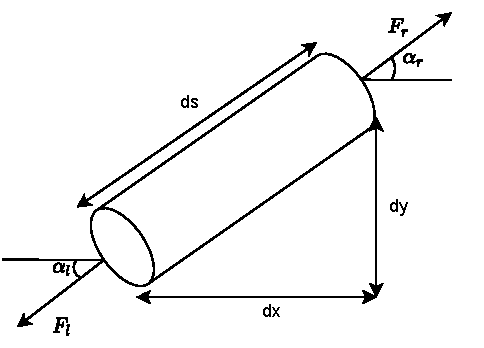
\includegraphics[width=0.7\linewidth]{touw_golf}
	\caption[Tijdsdomein analyse]{Tijdsdomein analyse PLACEHOLDER}
	\label{fig:tijdsdomein}
\end{figure}\\
We starten opnieuw met de algemene oplossing, maar dan op vaste plaats $x_1$:
\begin{align}
	y(x_1,t) &= y_msin(kx_1 \pm \omega t +\varphi)\\
	\label{eq:tijdsanalyse1}
	y(x_1,t) &= y_msin(\pm \omega t +\varphi_1)
\end{align}
met $\varphi_1 = kx_1 +\varphi$. We kunnen dit opnieuw doen voor $x_2$
\begin{align}
	y(x_2,t) &= y_msin(kx_2 \pm \omega t +\varphi)\\
	\label{eq:tijdsanalyse2}
	y(x_2,t) &= y_msin(\pm \omega t +\varphi_2)
\end{align}
We zien dus uit vergelijkingen \ref{eq:tijdsanalyse1} en \ref{eq:tijdsanalyse2}, dat er engel een fase verschuiving is. We vermelden ook nog dat oscillaties in fase zijn als $2\pi = k\lambda$.

We doen ook de analyse doen op de golfvergelijking in de ruimte:\\
\textcolor{red}{PLACEHOLDER}
\begin{figure}[h]
	\centering
	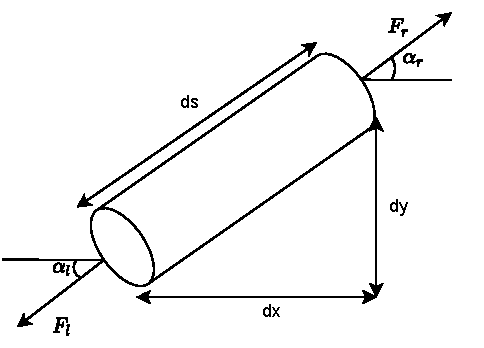
\includegraphics[width=0.7\linewidth]{touw_golf}
	\caption[Ruimtelijke analyse]{Ruimtelijke analyse PLACEHOLDER}
	\label{fig:ruimtelijkeanalyse}
\end{figure}\\
We starten opnieuw met de algemene oplossing, maar dan op vast tijdstip $t_1$:
\begin{align}
	y(x,t_1) &= y_msin(kx \pm \omega t_1 +\varphi)\\
	\label{eq:ruimteanalyse1}
	y(x,t_1) &= y_msin(kx +\varphi_1)
\end{align}
met $\varphi_1 = \varphi \pm \omega t_1$. We stellen dit opnieuw op voor $t_2$
\begin{align}
	y(x,t_2) &= y_msin(kx \pm \omega t_2 +\varphi)\\
	y(x,t_2) &= y_msin(kx \underbrace{\pm \omega t_1 +\varphi}_{\varphi_1}\pm\Delta t)\\
	\label{eq:ruimteanalyse2}
	y(x,t_2) &= y_msin(kx +\varphi_2)
\end{align}
met $\varphi_2 = \varphi_1\pm\Delta t$.
uit de waarden van $\varphi_1$ en $\varphi_2$ kunnen we de voortplantingsrichting van de golf bepalen: 
\begin{center}
	\begin{tabular}{|c|c|}
		\hline
		$\varphi_1$ < $\varphi_2$& Golf naar rechts \\
		\hline
		$\varphi_1$ > $\varphi_2$& Golf naar links \\
		\hline
	\end{tabular} 
\end{center}
We kunnen ook iets zeggen over de voortplantingssnelheid $v$.
\begin{align*}
 v = \frac{dx_{max}}{dt} = \frac{d}{dt}(kx_{max} \pm \omega t +\varphi) &= 0\\
 k\frac{dx_{max}}{dt}\pm \omega & = 0\\
 \pm \frac{\omega}{k} & = v\\
 \pm\frac{2\pi f}{\frac{2\pi}{\lambda}} & = v\\
 \pm \lambda f & = v
\end{align*}
\newpage
\section{Afleiding 9}
\textbf{Superpositie}\\
We zeggen dat de algemene oplossing $y(x,t)$ van de golfvergelijking kan uitgedrukt worden door 2 nieuwe functies:
\begin{equation*}
	y(x,t) = y_1(x,t)+y_2(x,t)
\end{equation*}
We vullen dit opnieuw in in de golfvergelijking:
\begin{align*}
	\frac{\partial^2 y(x,t)}{\partial t^2} & = v^2 \frac{\partial^2 y(x,t)}{\partial x^2}\\
	\frac{\partial^2 y_1(x,t)+y_2(x,t)}{\partial t^2} & = v^2 \frac{\partial^2 y_1(x,t)+y_2(x,t)}{\partial x^2}\\
\end{align*}
We gebruiken de lineariteit van de afgeleide:
\begin{equation*}
	\frac{\partial^2 y_1(x,t)}{\partial t^2} +\frac{\partial^2 y_2(x,t)}{\partial t^2}  = v^2(\frac{\partial^2 y_1(x,t)}{\partial x^2}+\frac{\partial^2 y_2(x,t)}{\partial x^2})
\end{equation*}
\end{document}
